\section{Results} % How well does the proposed solution perform?

% Compare the proposed solution against baseline and other solutions
%% Performance
%% Power
%% Area
%% Etc.
% Discuss the results
%% When and why does the proposed solution work well
%% When and why does the proposed solution work less well
\subsection{Sequential Prefetcher}
Testing a sequential prefetcher with a couple of different settings
for prefetch distance and prefetch degree. Results found in Figure~\ref{graph:seq}
\begin{figure}[h]
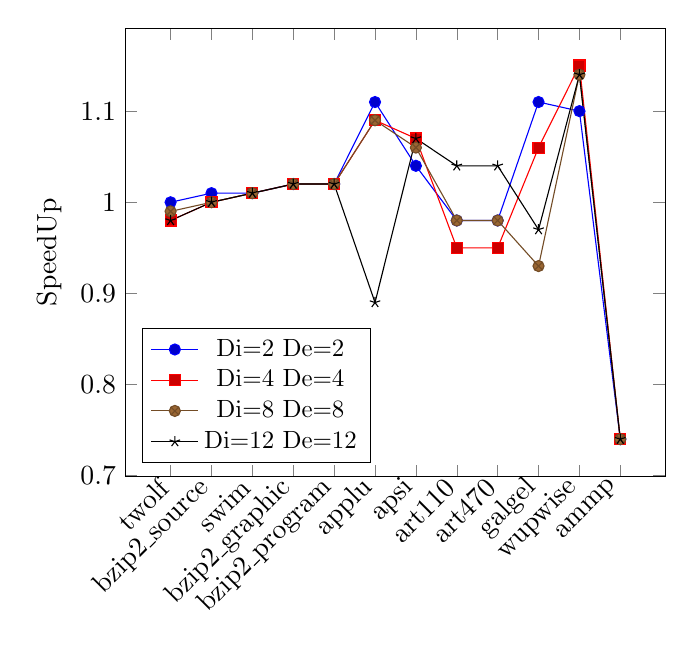
\begin{tikzpicture}
\begin{axis}[
    symbolic x
    coords={twolf,bzip2\_source,swim,bzip2\_graphic,bzip2\_program,applu,apsi,art110,art470,galgel,wupwise,ammp},
    xtick=data,
    x tick label style = {rotate=45,anchor=east},
    ylabel=SpeedUp,
    legend pos=south west,
    legend style = {nodes={scale=0.9, transform shape}}]
\addplot coordinates {
    (twolf,1.00)
    (bzip2\_source,1.01)
    (swim,1.01)
    (bzip2\_graphic,1.02)
    (bzip2\_program,1.02)
    (applu,1.11)
    (apsi,1.04)
    (art110,0.98)
    (art470,0.98)
    (galgel,1.11)
    (wupwise,1.10)
    (ammp,0.74)
};
    \addplot coordinates {
    (twolf,0.98)
    (bzip2\_source,1.00)
    (swim,1.01)
    (bzip2\_graphic,1.02)
    (bzip2\_program,1.02)
    (applu,1.09)
    (apsi,1.07)
    (art110,0.95)
    (art470,0.95)
    (galgel,1.06)
    (wupwise,1.15)
    (ammp,0.74)
};
    \addplot coordinates {
    (twolf,0.99)
    (bzip2\_source,1.00)
    (swim,1.01)
    (bzip2\_graphic,1.02)
    (bzip2\_program,1.02)
    (applu,1.09)
    (apsi,1.06)
    (art110,0.98)
    (art470,0.98)
    (galgel,0.93)
    (wupwise,1.14)
    (ammp,0.74)
};
    \addplot coordinates {
    (twolf,0.98)
    (bzip2\_source,1.00)
    (swim,1.01)
    (bzip2\_graphic,1.02)
    (bzip2\_program,1.02)
    (applu,0.89)
    (apsi,1.07)
    (art110,1.04)
    (art470,1.04)
    (galgel,0.97)
    (wupwise,1.14)
    (ammp,0.74)
};
\legend{Di=2 De=2,Di=4 De=4,Di=8 De=8,Di=12 De=12}
\end{axis}
\end{tikzpicture}
    \caption{Testing a sequential prefetcher with prefetch distance and degree set to 2, 4, 8 and 12.}
\label{graph:seq}
\end{figure}
\subsection{Overall Performance}
The overall tests showed an expected result. The more complex the prefetching
scheme, the higher the speedup compared to baseline as seen in
Figure~\ref{graph:base}. 
\begin{figure}[h]
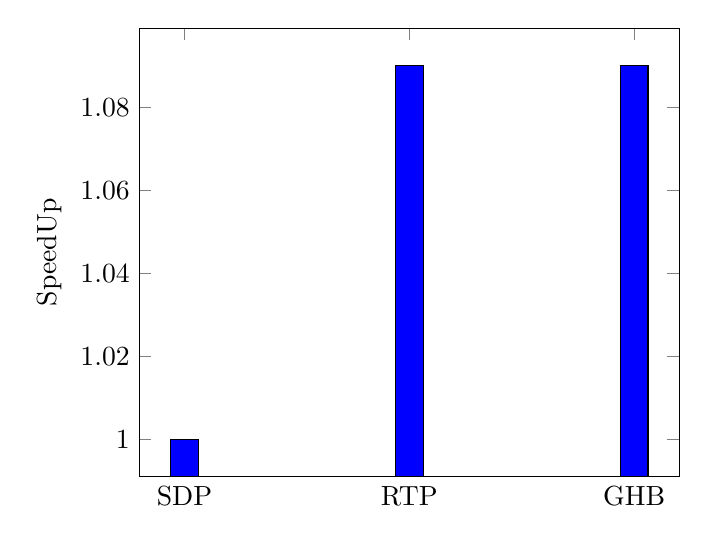
\begin{tikzpicture}
\begin{axis}[
    symbolic x coords={SDP,RTP,GHB},
    xtick=data,
    ylabel=SpeedUp
    ]
\addplot[ybar,fill=blue] coordinates {
    (SDP,1.00)
    (RTP,1.09)
    (GHB,1.09)
};
\end{axis}
\end{tikzpicture}
    \caption{Speedup of our implemented prefetchers compared to baseline.}
    \label{graph:base}
\end{figure}

\subsection{Test specific analysis}
We assesed the different prefetchers using the SPEC CPU2000 benchmark suite.
From Figure~\ref{graph:tests} it is clear that SDP does not success in creating
any difference while GHB and RPT have both large speed ups and slow downs with
an average on the positive side. They are very similar even if the
implementation is quite different.
\begin{figure}[h]
\begin{tikzpicture}
\begin{axis}[
    symbolic x
    coords={twolf,bzip2\_source,swim,bzip2\_graphic,bzip2\_program,applu,apsi,art110,art470,galgel,wupwise,ammp,blank},
    xtick=data,
    ybar interval=0.7,
    x tick label style = {rotate=45,anchor=east},
    ylabel=SpeedUp,
    legend pos=north west
    ]
\addplot[fill=gray] coordinates {
    (twolf,1.00)
    (bzip2\_source,1.00)
    (swim,1.00)
    (bzip2\_graphic,1.00)
    (bzip2\_program,1.00)
    (applu,0.99)
    (apsi,1.00)
    (art110,1.00)
    (art470,1.00)
    (galgel,1.00)
    (wupwise,1.00)
    (ammp,1.00)
    (blank,1)
};
    \addplot[fill=black] coordinates {
    (twolf,0.99)
    (bzip2\_source,1.00)
    (swim,1.01)
    (bzip2\_graphic,1.01)
    (bzip2\_program,1.04)
    (applu,1.05)
    (apsi,1.07)
    (art110,1.06)
    (art470,1.06)
    (galgel,1.09)
    (wupwise,1.25)
    (ammp,1.63)
    (blank,1)
};
    \addplot[black, fill=yellow] coordinates {
    (twolf,0.99)
    (bzip2\_source,1.00)
    (swim,1.01)
    (bzip2\_graphic,1.02)
    (bzip2\_program,1.04)
    (applu,1.05)
    (apsi,1.06)
    (art110,1.06)
    (art470,1.06)
    (galgel,1.11)
    (wupwise,1.25)
    (ammp,1.66)
    (blank,1)
};
\legend{SDP,GHB,RTP}
\end{axis}
\end{tikzpicture}
    \caption{Results for the tests in the SPEC CPU2000 benchmark suite.}
    \label{graph:tests}
\end{figure}
